\documentclass[comsoc,final]{IEEEtran}
\usepackage[utf8]{inputenc}
\usepackage[T1]{fontenc}
\usepackage[zerostyle=b]{newtxtt}
\usepackage{subcaption}
\usepackage[inline]{enumitem}
\usepackage{booktabs}
\usepackage{multirow}

\usepackage{graphicx}
\graphicspath{{figs/}}
\IEEEoverridecommandlockouts

\usepackage{amsmath,amssymb,amsfonts}
\usepackage{algorithmic}
\usepackage{textcomp}
\usepackage{xcolor}
\usepackage{lipsum}
\usepackage[english]{babel}
\usepackage{csquotes}

\newcommand{\todo}[1]{\textcolor{red}{#1}}

\usepackage{hyperref}
\hypersetup{
    colorlinks=true,
    linkcolor=blue,
    filecolor=magenta,      
    urlcolor=teal,
    pdftitle={Iscc2023 Paper}
}
\usepackage{xurl}


\usepackage[style=ieee,backend=biber,doi=false,url=true,maxnames=3]{biblatex}
\AtEveryBibitem{%
  \clearfield{note}%
}
\addbibresource{tebaka2023.bib}

\begin{document}    % 6 Pagine, Double Column

\title{\textsc{TEBAKA}: Territorial Basic Knowledge Acquisition. An Agritech Project for Italy: Results on Self-Supervised Semantic Segmentation}

\author{\IEEEauthorblockN{Lorenzo Epifani, Antonio Caruso\thanks{This work is financed by the European Union, PON Ricerca e Innovazione $2014-2020$, project TEBAKA, Fondo Sociale Europeo, Fondo Sociale di Sviluppo Regionale (FESN).}}\\ 
\IEEEauthorblockA{\textit{Dept. of Mathematics and Physics ``Ennio de Giorgi'', University of Salento, Lecce, Italy}}}

\maketitle



\begin{abstract}
Emerging technologies such as remote sensing from satellites and drones, 
internet of things (IoT), deep learning models, etc, could all be utilized to make informed and smart decisions aimed to increase crop production. We provide an overview of TEBAKA, an Italian national project on \emph{Smart Farming} and discuss its relevance in the overall scenario of similar projects. We emphasize the project originality, in particular the research activity on new data-driven ML models that better extract relevant knowledge from observations. We presented the task of \emph{image semantic segmentation} of olive trees or rows of grape plants and show an original self-supervised deep learning network that produce the segmentation with high accuracy. Furthermore, we discuss some idea that would be part of the project activities for the next year.
\end{abstract}

\begin{IEEEkeywords}
digital agriculture, precision agriculture, satellite images, deep learning, machine learning, sensor networks, IoT
\end{IEEEkeywords}


\section{Introduction}
% general intro to agritech and relevance for computer science.

The enabling technologies of distributed sensor networks, internet of things, remote sensing with multi-spectral cameras on satellites, drones and aerial platforms, together with smart decision support systems are key contributors for the emerging field of \emph{Digital Agriculture} (DA) or \emph{Agriculture 4.0} \cite{de2018agriculture}. 

The high-level goal is to support agronomist with \emph{Precision Agriculture} management practices, to better solve the challenges and demand like: an increasing world-population, rising production costs (like energy), labor shortages, and climate and environmental changes (like water resource scarcity). It leverages extensive knowledge acquisition using remote sensing technologies, and on-the-field deployment of sensors and IoT networks \cite{LiSurvey2021}%RAJ2021103107
and machine learning \cite{seng2018computer} to maximize resource usage and crop yield while minimizing associated costs.

In the United States, the use of yield-maps and soil maps are adopted only by 5 to 25 percent of total U.S. farms; on the other hand automated guidance has increased sharply, with the advance in deep-learning applied to computer vision, and it is applied to over 50 percent of the cultivated areas. A good survey of the trend in the technology evolution of a \emph{Smart Farm} in the USA is in \cite{mcfadden2023precision}. USDA (The U.S. Department of Agriculture) is investing up to $2.8$ billion in $70$ selected projects under the first Partnerships for Climate-Smart Commodities funding pool, as a part of the Inflation Reduction Act.

\begin{figure}
    \centering
    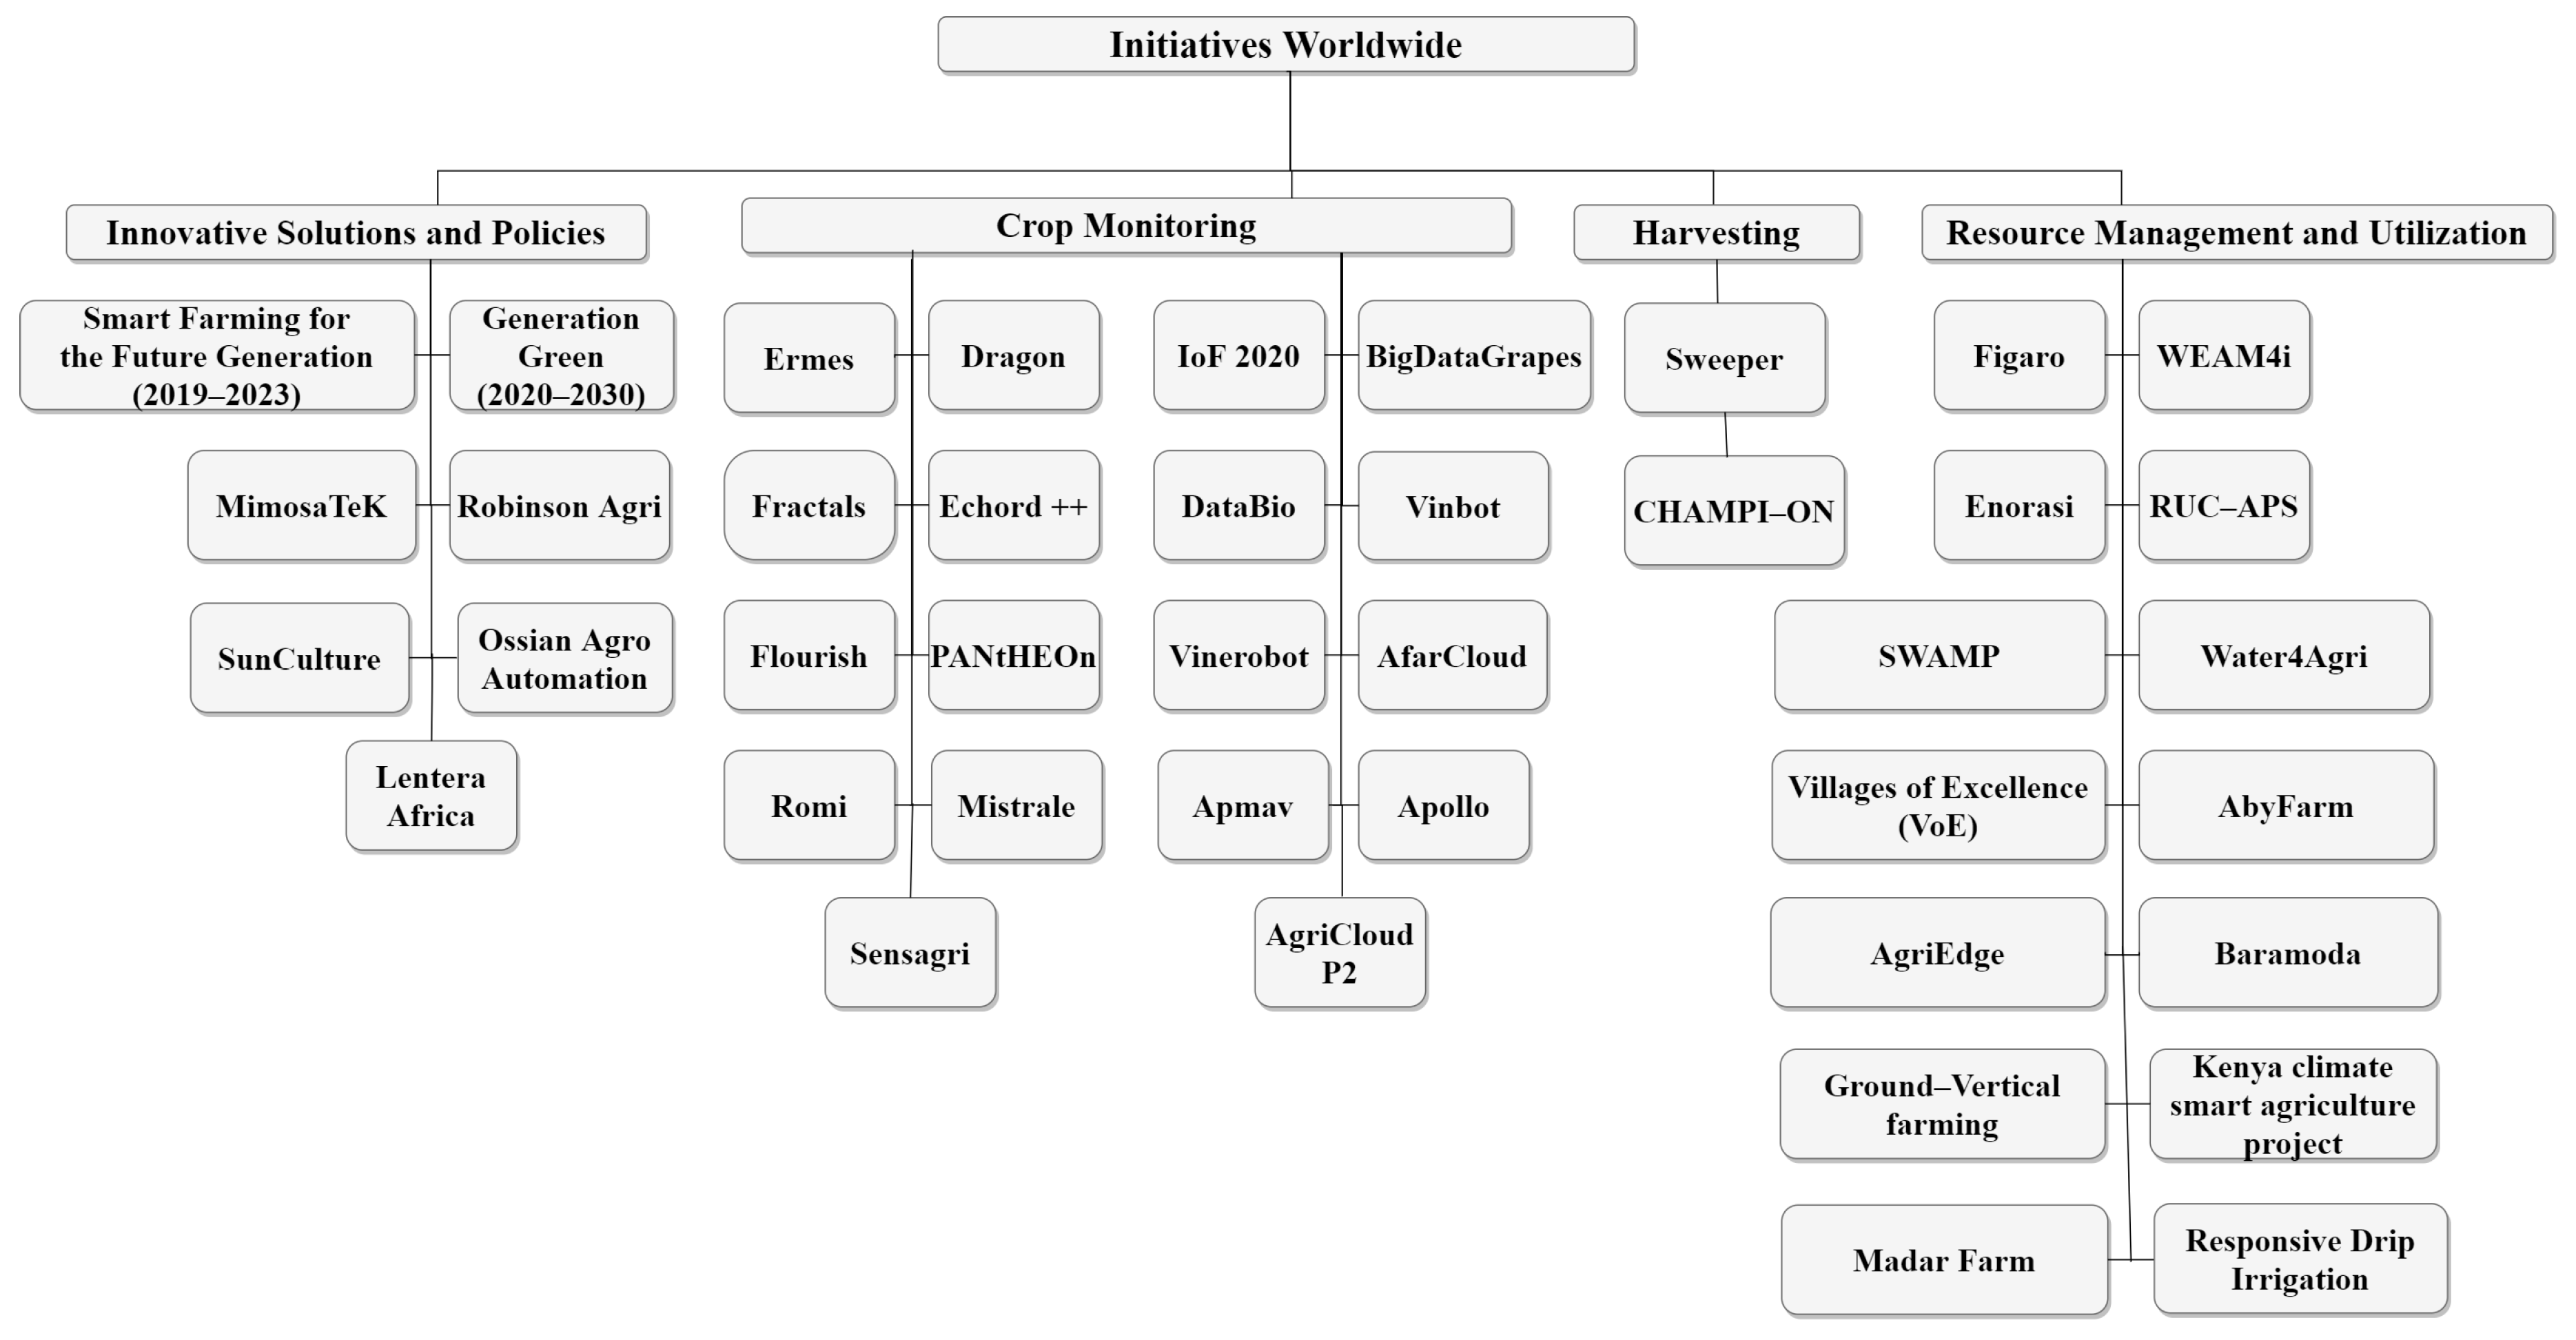
\includegraphics[width=\columnwidth]{agriengineering-04-00029-g005}
    \caption{A classification of active European Union funded projects in the area of Digital Agriculture (from \cite{agriengineering4020029})}
    \label{fig:euprojects}
\end{figure}

In Europe, the European Community has funded many projects that integrate ICT technologies and Digital Agriculture, we see in Figure \ref{fig:euprojects} a collection of active research project and startups, classified in different areas, such as:  \emph{Crop Monitoring}  (the largest one), \emph{Harvesting}, optimization of \emph{Resource Managements} and \emph{Innovative Policies and Solutions} with more than $41$ initiatives. In Table \ref{fig:table-worldwide} another list of worldwide projects that are actually funded, with a increasing role for African and Middle-East countries.

In this paper, we present the activities of \textsc{TEBAKA}: a national project funded by PON-FESN (European Union Social Fund) dedicated to develop the adoption of Digital Agriculture in the south part of Italy (Mezzogiorno) and in particular in Apulia (Puglia). The project span four years, from 2020 to 2024 and with an overall budget of 6.2 Million Euro it put together 10 partners from industry, universities, several national research institutions of Italian CNR, and private partners with a mixed background (someone more oriented to ICT services, someone more related to agronomy). 
We discuss the project in the following section, but we want to summarize here the key ideas involved. The project goals are a new generation of decision support systems, for agronomists, for the culture of grain, vine and olive. For this goal, the project comprise a large campaign of data acquisition, with measurements taken directly on the culture and soil, spanning two full year. Moreover, all measurements will be taken at the same time of the observations made with satellites  (Sentinel 2, Planet, ESA), and drones, aircraft equipped with a multi-spectral camera. These four levels of observation are unique in all the projects presented in the previous discussion, they allow a \emph{pyramidal representation} at different spatial resolution of the observed phenomena, repeated also, in different time. On top of this raw observations, we develop data-driven models (mostly based on \emph{neural networks}) that extract features from images related with the specific conditions of the annual crop life cycle.

The rest of the paper is organized as follows: in \ref{sec:tebaka} we review the project structure and goals and actual status; in \ref{sec:activities} we present some interesting original results. An important task in the overall pipeline of analysis is a proper \emph{semantic segmentation} of the plant crown (foliage), i.e a mask that label each pixel of an image taken from UAV, as 'terrain' or 'green area'. We present an original self-supervised approach to the problem, and discuss the results, in \ref{sec:related} we collected some related works, and finally we have drawn in \ref{sec:conclusion} the conclusions.

\begin{figure}
    \centering
    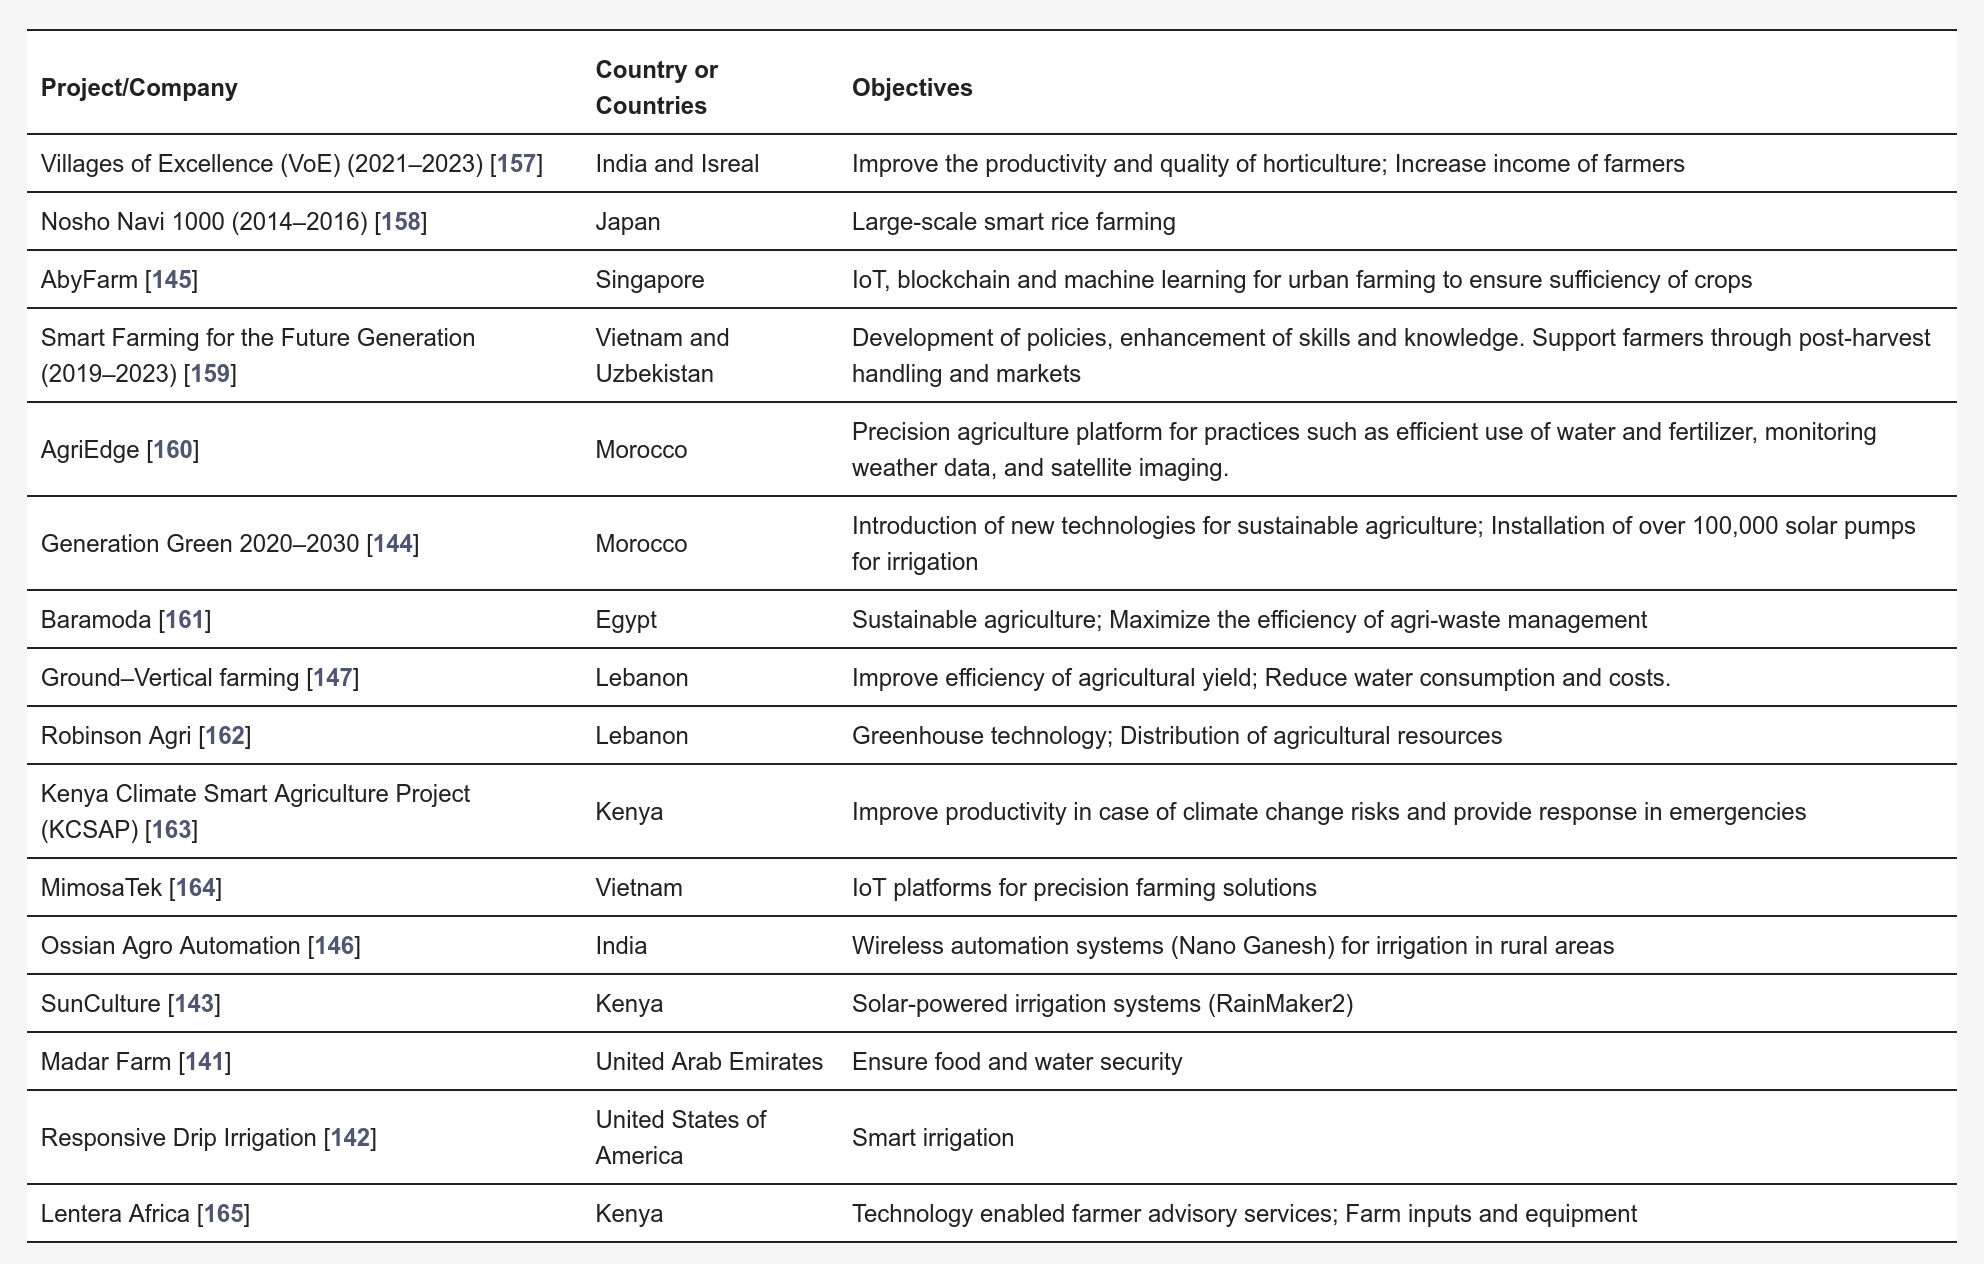
\includegraphics[width=\columnwidth]{research-table}
    \caption{A list of worldwide projects related to the area of Digital Agriculture (from \cite{agriengineering4020029})}
    \label{fig:table-worldwide}
\end{figure}

%--------- end of intro

\section{Tebaka Project Description}\label{sec:tebaka}

TEBAKA stands for \emph{Territorial Basic Knowledge Acquisition}, i.e. a  “\emph{platform}” focused on the analysis of the phenological cycle of grain, vines and olive, all of which are significantly present in the south of Italy. It will operate through $3$ phases, articulated in almost four year, from November 2020 to April 2024, with different sub-tasks. We describe in the following the most important ones.\medskip

\textsc{Data Acquisition:} One of the largest and complex task in TEBAKA is organizing a multi-year plan of observation from different \emph{sources} in order to capture at least two different year of crops grow. The source of data, must be synchronized in order to operate at the same date, to obtain for each observed point a \emph{pyramidal} view at the different resolutions. The data comes from: classic environmental stations on the field, manual sampling  of chemical and physical properties of soil and plant in specific points (operated by agronomist), satellite images (Sentinel, Planet), drone images and aircraft images. We identified three areas of interest, one for each different culture, and obtained the authorizations to operate with aircraft and drones. A computational and storage system based on Open Data Cube \cite{odc} has been put in place in order to collect all the observations and provide an interface for cloud computation on a large cluster\footnote{The Open Data Cube provide a JupyterHub instance to run any Python code, all the result in the paper has been obtained using Pytorch or custom scripts.}. The first year of observations has been completed in 2022, while the second phase will start this spring.\medskip

\textsc{Analysis and Modelling Phase:} This is clearly the larger task in the project, with the goal of developing new advanced models that transform the knowledge extracted from the data, in new precision agriculture (data-based) management practice on the field. 
Major sub-tasks are: models of the annual production cycles of the agricultural crops considered, fusion criteria of data from multi-sensory sources, data driven models for image analysis, image segmentation to identify homogeneous area in images, change detection to measure and/or predict the regular/irregular grows of the plants.\medskip 

\textsc{Prototype Development:} In this task, the partner will contribute in order to develop a prototype of an integrated platform composed of (1) observational services (unmanned or manned aircraft, drones, satellite) that can be acquired from intermediate or final users to get new data each season, for their area of interest, (2) a portfolio of data-driven models that works as the engine inside, one or more, decision support system, used by the final user, exposed thought standard REST services. 

In the next section, we present a result obtained in the second phase of the project (i.e. modelling) on a data driven model to solve the task of \emph{image segmentation} in order to label the green areas (i.e. foliage, leaf) of an image.
%% ------------------------------- ciccia ---------------

\section{Self-Supervised Semantic Segmentation of Plant Crown}\label{sec:activities}
% Image analysis using deep learning, role, goals result.

Segmentation is a recurrent task in literature regarding precision agriculture: the information provided by a pixel-wise classification map can by used to solve different domain specific tasks \cite{s21051617,rs14061523,Egli20201} like: biovolume estimation, tree crowns mapping, estimate the distribution of the population for different species, monitoring changes in green areas. In particular we are interested in a measure of the \emph{volumetric leaf area} and its evolution across time.

The two main remote sensing technologies that have been used over the years are satellite and UAV imagery, each one having his pros and cons. Even if satellite imagery has also been used successfully by several authors \cite{ruswurm_multi-temporal_2018, daudt_fully_2018, ienco_land_2017}, the unmanned aerial vehicles (UAVs) have proven to be a game-changing technology for various reasons \cite{Adao2017}. The main one is that for the majority of agriculture challenges, there are strict resolution requirements that satellite imagery cannot satisfy. These requirements can be meet by UAV imagery while keeping costs acceptable. Satellite imagery is the best choice only if we have to deal with large scale observable phenomena \cite{gurumurthy_mango_2019,guirado_mask_2021}, since specific patterns can be observed only from a certain scale onward. For these reasons, we decided to choose UAV imagery as data source.

In agronomy, there are many well known \emph{spectral indexes} that are used to assign a score to each pixel. These indexes are often linear (or non-linear) combination of spectral channels, and have proven to be highly correlated to specific characteristics available in areas that have a value of the index above a threshold. The \emph{Normalized Difference Vegetation Index} (NDVI) is an index, whose formula is:

\[ NDVI = \frac{NIR-R}{NIR+R} \]

The choice of these two light bands is based on the fact that plants absorb light energy in the red band for chlorophyll photosynthesis and instead reflect a lot of energy in the near-infrared band due to the cell structure of the plants themselves. Therefore, the NDVI exploits these properties to measure the amount of chlorophyll and foliage density present in vegetation. The index ranges from a value of -1 to +1, where a value of -1 indicates the presence of water or snow, 0 indicates an unvegetated surface such as rocks or bare soil, and a value of +1 indicates extremely dense vegetation. In general, higher NDVI values correspond to higher vegetation density and plant health.

Even if NDVI thresholding can be used to produce a segmentation map of an UAV image, there are many issues that make it a non-optimal choice. Different objects with the same spectrum obtains the same score, even if they belong to different classes. Moreover, NDVI does not consider local properties and patterns. So, simple thresholding is insufficient, and image analysis through deep learning has proven to provide state-of-the-art solutions for instance/semantic segmentation in different domains \cite{moen_deep_2019,garcia-garcia_review_2017}. For this reason, this method has been widely used in precision agriculture in the last decade \cite{bouguettaya_deep_2022}.

However, supervised deep learning methods require large, hand-labelled datasets, that are carefully prepared by domain experts. In fact, in all the works examined, and reviewed in the next section, the labelling is carried out by agronomists. In this work, we propose an original solution for the automatic labeling of UAV images containing vineyards and olive trees. We tested this method, by using this data-set to train a well-known semantic-segmentation neural network model, the entire system can be considered a self-supervised model, with the advantage that the self-labelling pipeline, can be used to label any plant species without the costly manual labor of a domain expert (in this case an agronomist). To the best of our knowledge, there is no other work using a similar solution in this domain, in particular we are not aware of a single method that can be used on more than a single culture type. 

The self supervised pipeline is a system that takes as input a hyper-spectral orthomosaic and returns the set $\mathcal{D}$: \[
\mathcal{D} = \{\, (\overline{x}_i,\overline{y}_i):i \in \{1...N\}\,\}
\] where $\overline{x}_i$ represents the $i$-th tile of the input orthomosaic, $\overline{y}_i$ is the ground truth mask for $\overline{x}_i$ and $N$ is the total number of collected tiles i.e. the size of the dataset.
Masks and tiles have the same spatial resolution, but masks have only one channel, with the value of each pixel be equal to 0 (background) or 1 (vegetation). During the development of the machine learning model, we represented the two values with the one-hot-encoding method.
Only
two classes have been assigned to speed up prototyping, but their number can be easily extended, i.e. by labelling each species with a different value. The self supervised pipeline (Figure \ref{fig:entirepipeline}) works as follow:

\begin{figure}
    \centering
    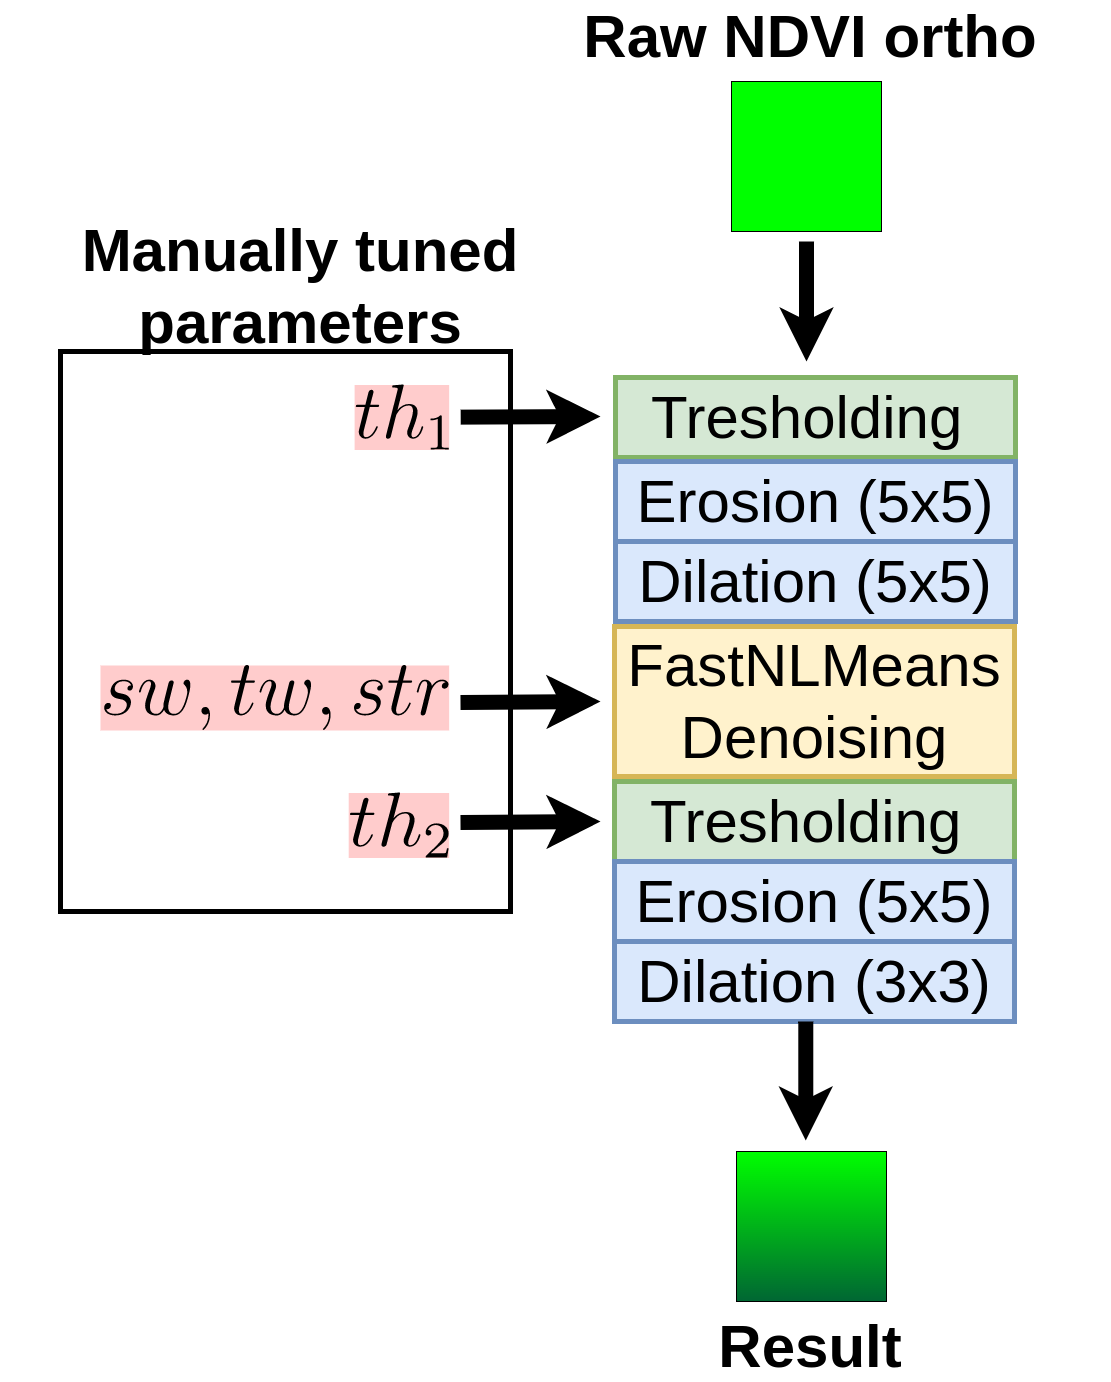
\includegraphics[width=0.75\columnwidth]{tunable_module}
    \caption{Schema of the Tunable Denoising Module.}
    \label{fig:tunable_module}
\end{figure}%

\begin{figure}
    \centering
    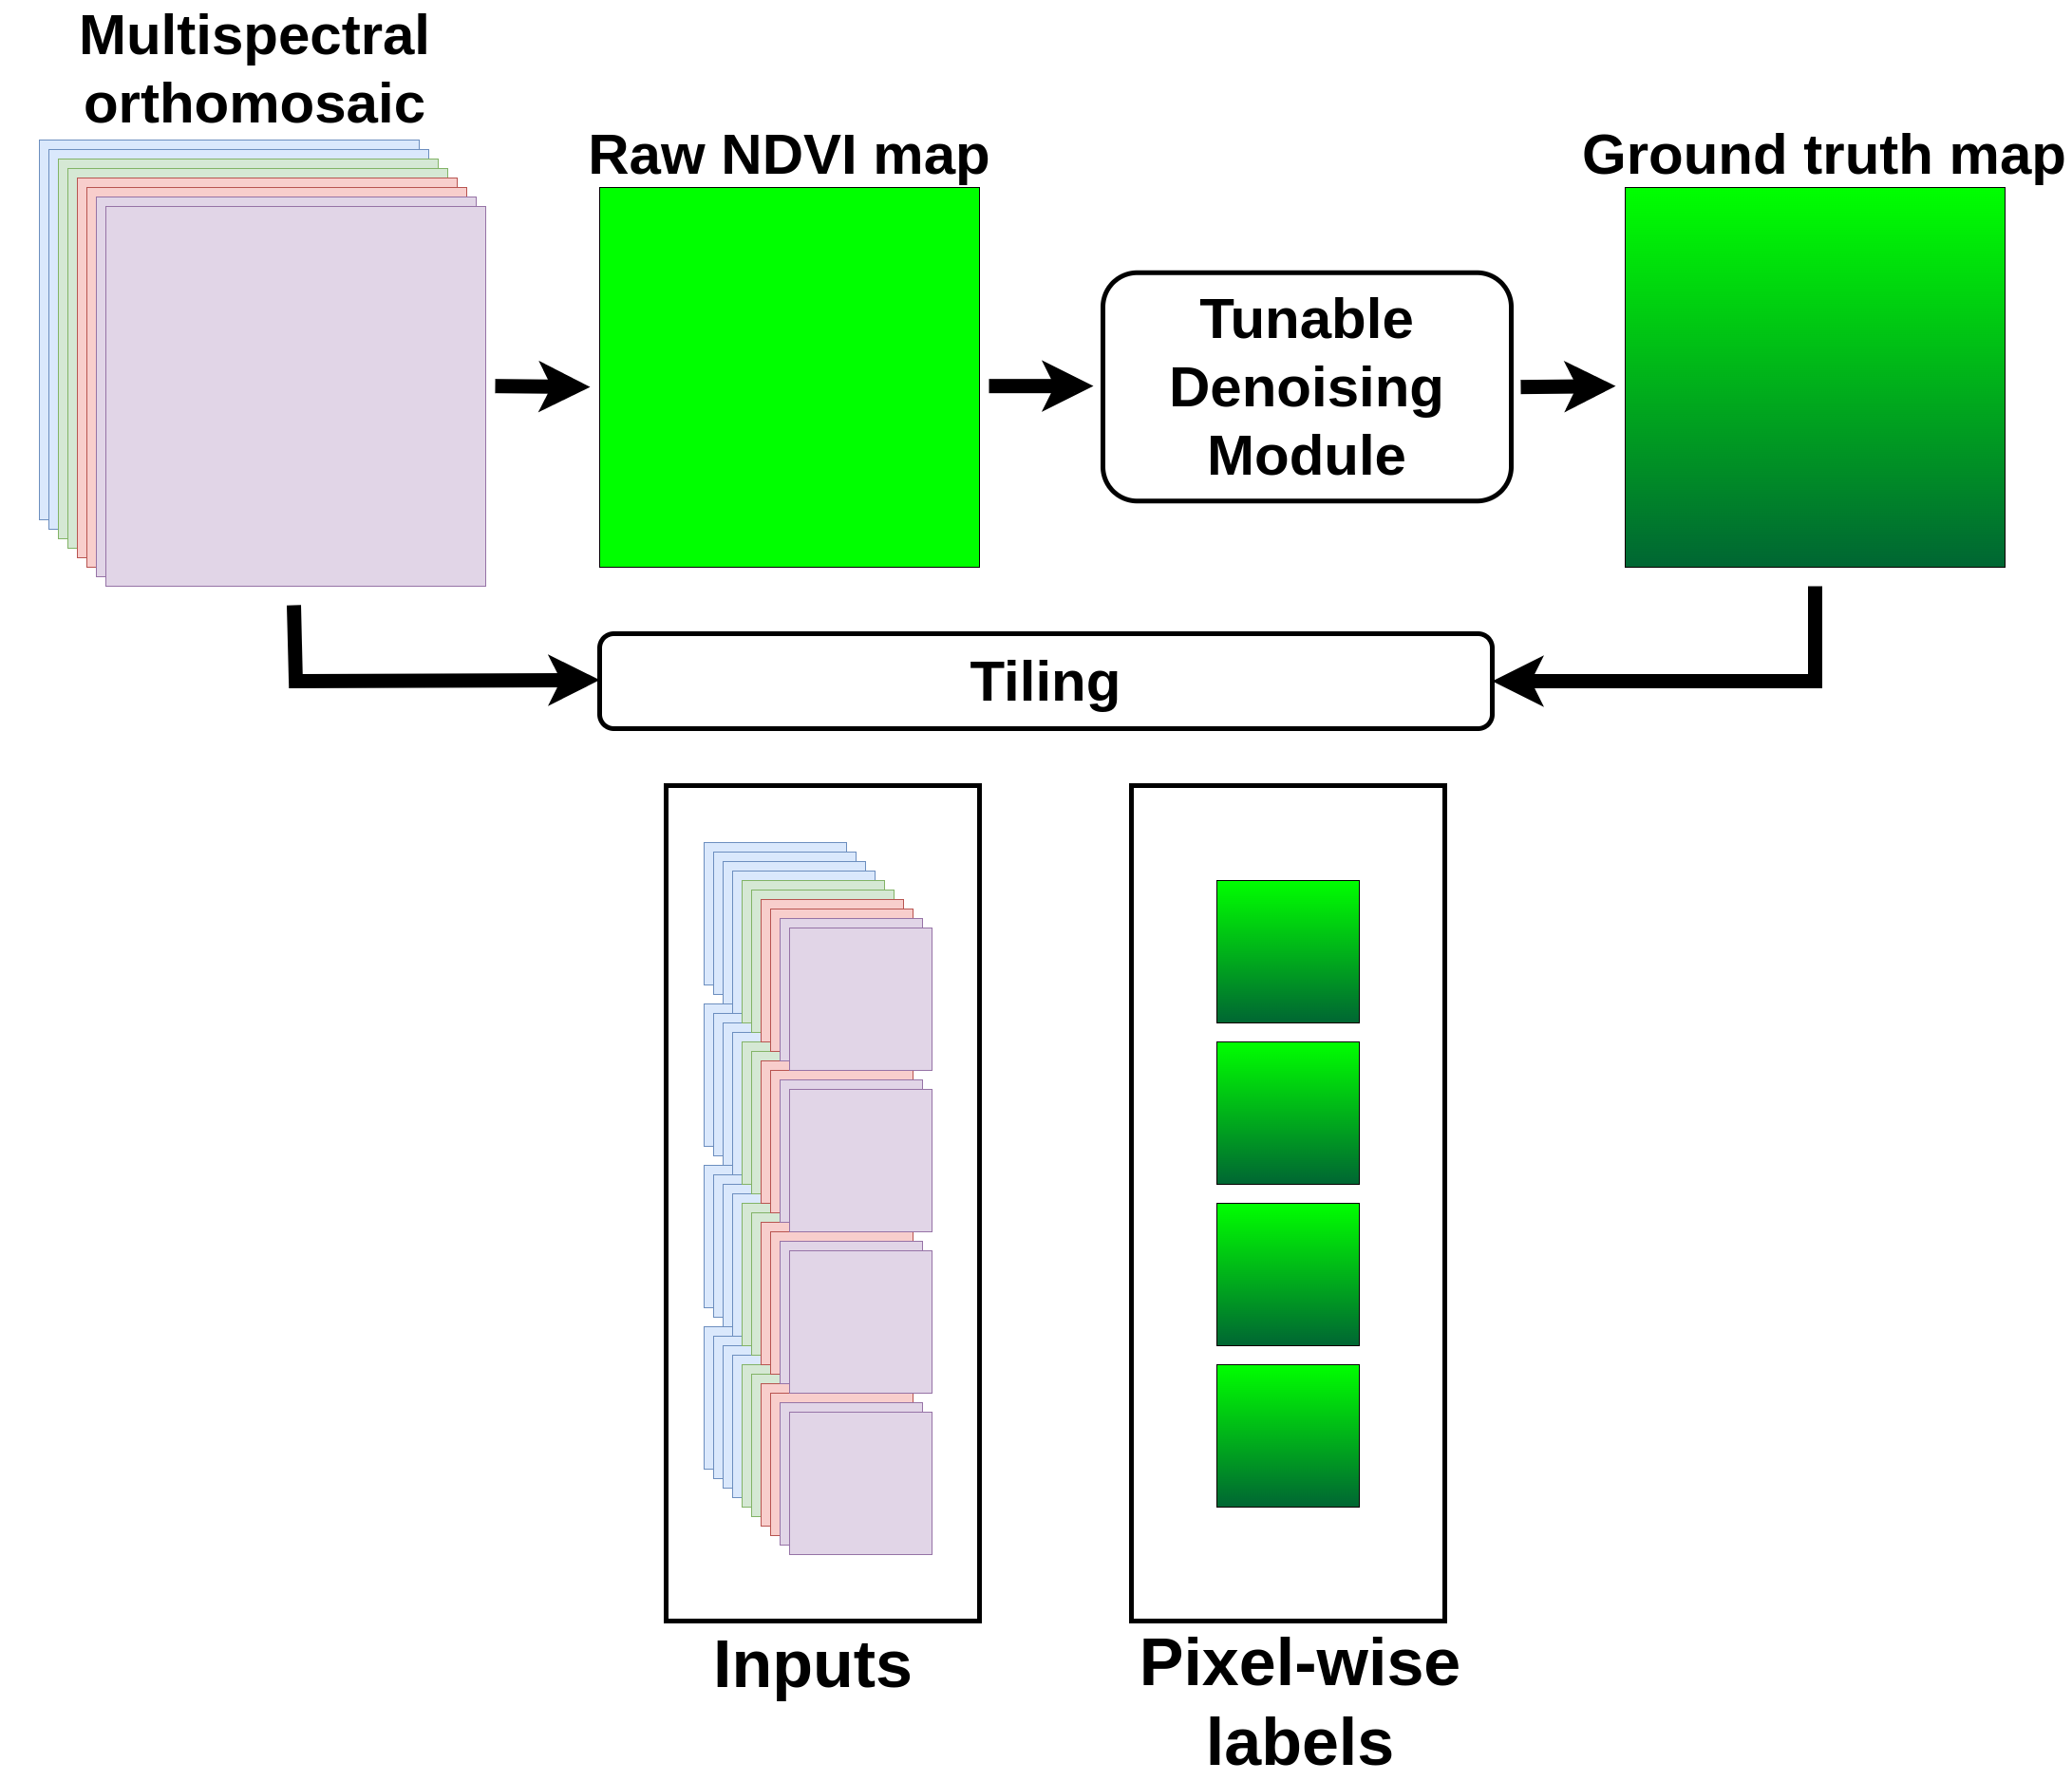
\includegraphics[width=0.75\columnwidth]{pipeline1}
    \caption{Graphical representation of the entire self-supervised pipeline.}
    \label{fig:entirepipeline}
\end{figure}%

\begin{itemize}
    \item The NDVI is computed pixel-wise from the multispectral input orthomosaic and stored as a single-channel image. 
    $NIR$ (Near Infra Red) and $R$ (Red) bands are respectively stored in the 10th and the 6th channels of our source orthomosaic.
    \item The NDVI map is the input to a Tunable Denoising Module that is part of the self-supervised model. This component (shown in Figure \ref{fig:tunable_module}) is a stack of different well known image processing techniques executed sequentially. 
    The module is executed by fixing a set of parameters that govern its operation. In our experiments, the values of these parameters were found by drawing inspiration from the search criteria for hyperparameters used in machine learning (e.g. grid search inside intervals considered reasonable).
    This module produces the pixel-wise ground truth map for the entire hyperspectral source orthomosaic. The tunable parameters of this module are 5 (highlighted in red in previous image). Values $th_1$ and $th_2$ governs the two thresholding stages, while $sw$, $tw$ and $str$ respectively represents the search window size, the template window size and the strength of the fast non-local means denoising method. For the dilation and the erosion, we used kernels containing only 1 with size $3\times3$ and $5\times5$.
    An erosion followed by a dilation is called opening. The opening is a smoothing filter and the specific behavior depends on the kernel size and content. An opening preserve as much as possible regions having similar structure respect to the kernel, while removing those different. Our kernels with all 1's allow to remove isolated groups of pixels, while their dimension governs the minimum size that groups of pixels must have in order to be preserved. Kernel size and content could be governed introducing some parameters, although in our experiments we achieved good results with fixed kernels.
    In our case, they serve to remove groups of isolated pixels classified as plants.
    \item The orthomosaic/ground truth are both split in many tiles of a fixed size. We pairwise store each input tile and its corresponding ground truth tile. The size of the tiles was chosen consistently with the size of the input expected from the semantic segmentation deep learning model we trained.
\end{itemize}

Before storage, pairs of tiles containing insufficient vegetation are discarded.
Formally, we can write the truth map $y_i$ as a matrix:
\[
\overline{y}_i=\begin{pmatrix}
  y_{1,1} & y_{1,2} & ... &y_{1,M}\\ 
  y_{2,1} & y_{2,2} & ...&y_{2,M}\\
    ... & ... & ...& ...\\
    ... & ... & ...&y_{M,M}\\
\end{pmatrix};\,\, y_{j,k}\in\{0,1\}
\]
Where, in our case, $M=388$. After that, we fix a threshold for the minimum ratio for vegetation-labelled pixels, called $th_{veg}\in[0,1]$. If, for a specific $\overline{y}_i$ the following statement is verified:\[
\frac{\sum_{j}^N\sum_{k}^N y_{j,k}}{M^2}< th_{veg}
\] 
then the pair $(\overline{x}_i,\overline{y}_i)$ is discarded.
This was done to prevent samples containing many background pixels from overpowering those with pixels labelled as vegetation. 
In our experiments, we labeled $906$ tiles (net of rejected ones) starting from $5$ UAV orthomosaics acquired in $2$ different areas of interest.

\begin{table}[htbp]
  \centering
  \caption{Areas of interest}
  \label{tab:aoi}
  \begin{tabular}{c*{3}{c}}
\toprule
           & GSD     & Area (km$^2$)             & \# Flights  \\
    \midrule
    Area-0  & $10$cm/px& 0.072 & $3$  \\
    \cmidrule(l{0.5em}r{0.5em}){1-4}
    Area-1 & $3$cm/px & 0.005 & $ 2 $  \\
    \bottomrule
  \end{tabular}
\end{table}

Flights for the acquisition were performed in a temporal window spacing from the $26$ May $2022$ to $30$ Sep $2022$.
All the acquired orthomosaics are 10-channel multi-spectral.
The model of neural network that used is the U-Net \cite{ronneberger_u-net_2015}, with some modifications, for example making it capable of handling the 10 channels for the multi-spectral images in input. 
Tiles have a resolution of $572\times572$ pixel. The U-Net is able to classify the inner square having size $388\times388$ because it needs to evaluate the context around each pixel, leaving the pixels on the edge unclassified. However, it is possible to classify the entire orthomosaic by properly managing a sliding window and applying mirroring to the border tiles of the orthomosaic. The patches represent areas of 327 m$^2$  and $98$ m$^2$ for their respective areas of interest, according to spatial resolution of the orthomosaics from which they are sampled.

We chose the U-Net over other similar architectures for several reasons: it has fewer parameters than competing networks, moreover, it was originally proposed to solve a task of similar complexity (biomedical image segmentation) with excellent results, which were then replicated on use cases very similar to ours. Lastly, in these publications (and also in the original work) the U-Net was trained from scratch with datasets of comparable size to ours (often even smaller).

We performed several training runs in order to cross validate different hyperparameters: decay rate, learning rate, number of epochs, and batch size. We listed in table \ref{tab:hyperpar}, the best 3 models chosen from all those tested in cross-validation, and in Figure \ref{fig:unet_models} we show how these models behave in inference.

\begin{figure}{\centering%
      \begin{subfigure}[b]{0.47\columnwidth}
         \centering 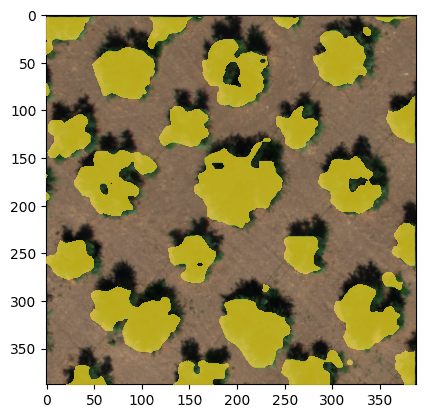
\includegraphics[width=\columnwidth]{ULIVO0INF}
     \end{subfigure}%
%
      \begin{subfigure}[b]{0.47\columnwidth}
         \centering 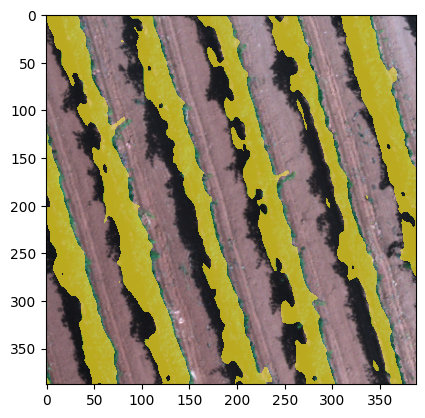
\includegraphics[width=\columnwidth]{VITE0INF}
     \end{subfigure}}
%       
      \begin{subfigure}[b]{0.47\columnwidth}
         \centering 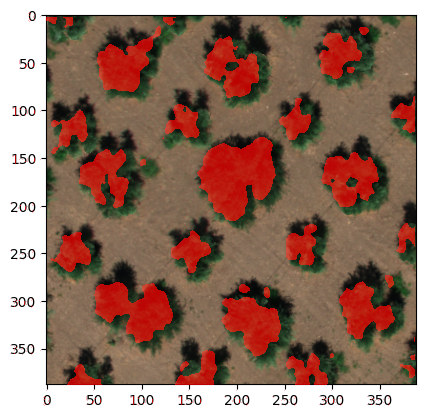
\includegraphics[width=\columnwidth]{ULIVO1INF}
     \end{subfigure}%
% 
      \begin{subfigure}[b]{0.47\columnwidth}
         \centering 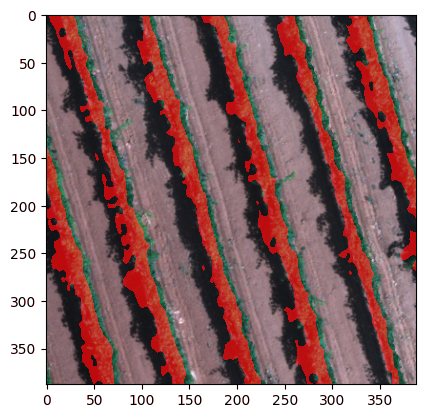
\includegraphics[width=\columnwidth]{VITE1INF}
     \end{subfigure}
%
      \begin{subfigure}[b]{0.47\columnwidth}
         \centering 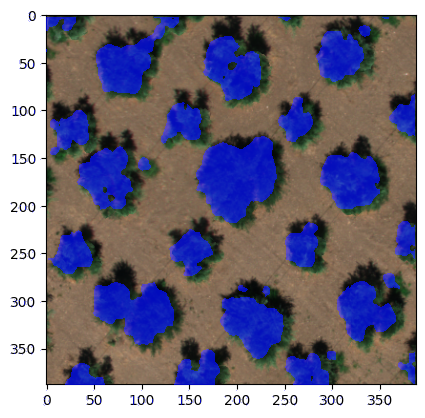
\includegraphics[width=\columnwidth]{ULIVO2INF}
     \end{subfigure}%
%       
      \begin{subfigure}[b]{0.47\columnwidth}
         \centering 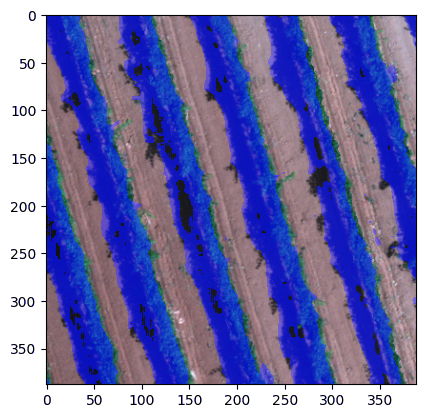
\includegraphics[width=\columnwidth]{VITE2INF}
     \end{subfigure}%
     \caption{Overlay between the input tiles and the result produced by our models. Yellow is for model-0, red for model-1 and blue for model-2.}
     \label{fig:unet_models}
\end{figure}


\begin{table}[htbp]
  \centering
  \caption{Hyperparameters settings \label{tab:hyperpar}}

  \begin{tabular}{c*{5}{c}}
    \toprule
    & \multirow{2}{*}{\shortstack{Learning\\rate}} & \multirow{2}{*}{\shortstack{Decay\\rate}}  & \multirow{2}{*}{\shortstack{Decay\\ each}} & \multirow{2}{*}{\shortstack{Epochs}} & \multirow{2}{*}{\shortstack{Batch\\size}} \\\\
    \midrule
    Model-0  & $5\cdot10^{-4}$ & $0.75$ & $40$ & $4$ & $5$ \\
    \cmidrule(l{0.5em}r{0.5em}){1-6}
    Model-1 & $5\cdot10^{-4}$ & $0.75$ & $40$ & 2 & 10 \\
    \cmidrule(l{0.5em}r{0.5em}){1-6}
    Model-2 & $5\cdot10^{-4}$ & $0.95$ & $20$ & 25 & 10 \\
    \bottomrule
  \end{tabular}
\end{table}

An usual metric that drive the learning phase and measure the quality of a segmentation task is IoU \emph{intersection over union}. We decided to avoid this measure since our self-supervised labelling system represents an approximation of the true labels, thus in some cases, it introduce errors, for example, in Figure \ref{fig:input_gt} we shown how it label shadows as vegetation in the case of vineyard. 

\begin{figure}{\centering%
%
      \begin{subfigure}[b]{0.47\columnwidth}
         \centering
         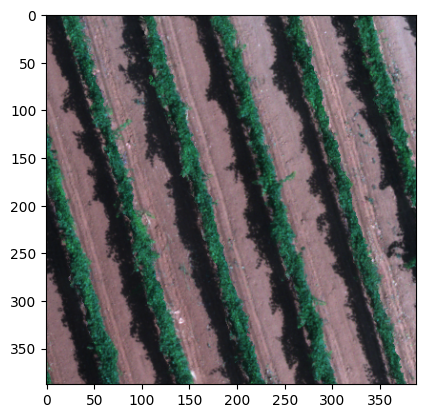
\includegraphics[width=\columnwidth]{vite}
         \caption{}
         \label{maskplot:a}
     \end{subfigure}%
%
     \begin{subfigure}[b]{0.47\columnwidth}
         \centering
         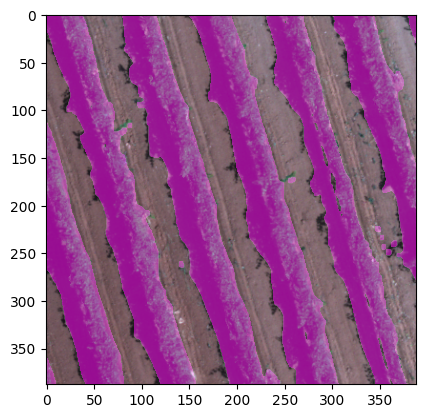
\includegraphics[width=\columnwidth]{vite_GT}
         \caption{}
         \label{maskplot:b}
     \end{subfigure}}\hfill
%       
     \begin{subfigure}[b]{0.47\columnwidth}
         \centering
         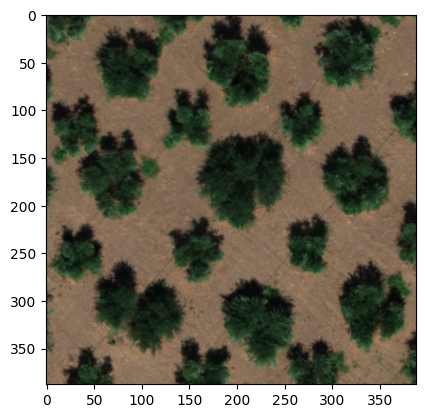
\includegraphics[width=\columnwidth]{ulivo}
         \caption{}
         \label{maskplot:c}
     \end{subfigure}%
%
     \begin{subfigure}[b]{0.47\columnwidth}
         \centering
         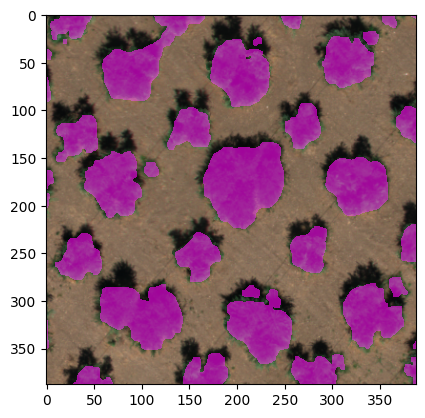
\includegraphics[width=\columnwidth]{ulivo_GT}
         \caption{}
         \label{maskplot:d}
     \end{subfigure}%
%        
     \caption{(a) Inner square of an input tile, vineyard; (b) Overlay between the previous input tile and the result produced by our self supervised pipeline; 
     %(c) Overlay between the vineyard input tile and his ground truth mask. 
     (c), (d) are the same but for olive trees.}
     % don't break lines manually NEVER
     \label{fig:input_gt}%
\end{figure}

 Despite this, some of our trained U-Net models are unaffected by this error (especially model-1) and can distinguish crowns from shadows. The reader can observe that although model-1 is visually better than model-2 (Figure \ref{fig:unet_models}), a comparison with any metric would lead us astray as error is also present in the ground truth masks.

In our experiments, some models are able to generalize well because not all shadows are labelled as vegetation (especially in olive trees, but this also happens in many portions of vineyard). Models that are trained for too many epochs tend to overfit and label shadows as vegetation. This is especially evident in the case of vineyard.
This problem can be handled when generating the dataset by introducing asymmetrical opening kernels, in order to perform stronger erosion in the direction in which the shadow is present and/or weakening dilation in the same direction. This would add parameters to the self-supervised pipeline, increasing its complexity and the time required for fine-tuning. From the discussion above we see that, the solution presented is viable, and solve the task of semantic segmentation even without a proper labelled dataset.



\section{Related Works}\label{sec:related}
%\todo{Completiamo, non creare frasi troppo brevi e sconnesse. inserisci i riferimenti, domani prima di caricare il pdf su EDAS sentiamoci.}

Although the surveyed works exhibit significant heterogeneity, several commonalities can be identified. Each author has a different area of interest, with its own local characteristics and species, and therefore everyone provides for themselves in the construction of the dataset. In general, almost all authors perform 3 steps in common: acquisition of raw data with planned UAV flights, orthomosaics tiling and manual labelling performed by domain experts.

%Safonova et al in \cite{s21051617} proposed a Mask R-CNN implementation to solve an instance segmentation task. In this work, they used the Mask R-CNN model to identify (with 2 different classes) shadows and crowns of several olive trees featured in an orthomosaic. The shadow was used to estimate the height of each tree. 
Safonova et al. \cite{s21051617} proposed a Mask R-CNN implementation to classify shadows and crowns of olive trees, the shadow information was used to estimate the height of each tree.
From the height estimation, it was possible to estimate the biovolume of the trees, which value was measured for 6 trees and used to evaluate the performance of the entire pipeline. The resulting model estimate the biovolume with an error of no more than 10\% of the measured values.%
%
%Ye et. al. in \cite{rs14061523} proposed an implementation of a stacked U-Net (also called U$^2$-Net) to solve a binary semantic segmentation task. The goal was to separate olive crown surface from the background. The nested structure of the chosen architecture has shown a great potential in capturing multiscale feature information.
 Ye et al. \cite{rs14061523} proposed a stacked U-Net (also known as U$^2$-Net) for semantic segmentation of olive crown surfaces. This approach leverages the nested structure of the chosen architecture which has shown a great potential in capturing mult-iscale feature information.
%Gurumurthy et al in \cite{gurumurthy_mango_2019} proposed a fully convolutional neural network for the instance segmentation of mango trees. This work aims to the individual crown detection in the target crop. Their approach is different: the selected model is first trained for the semantic segmentation of tree crowns. At this stage, the network produces a single map of scalars, each value of the map represents a score describing the probability that the observed pixel belongs to a canopy. In the next stage, the network is retrained by replacing the head so that it produces a map with the scores of 3 different classes. In this case, the classes represent the canopy, the background, and the intersection surface between the canopies. The two training steps use a differently labeled dataset.
Gurumurthy et al. \cite{gurumurthy_mango_2019} presented a fully convolutional U-Net inspired neural network for instance segmentation of mango trees, aiming to detect individual instances of tree crowns in the target crop. Their approach is to first train the chosen model for semantic segmentation of tree crowns, producing a single map of scalar values representing the probability that an observed pixel belongs to a canopy. Next, the network is retrained to produce a map with scores for three different classes: canopy, background, and the intersection surface between canopies. These training steps use differently labeled datasets.
%Natesan et al. in \cite{Natesan2019475} proposed a Resnet 50-based CNN to classify patches containing tree crowns into 3 different classes (red pine, white pine, non-pine). Patches were extracted from an orthomosaic using a processing pipeline based on classical computer vision techniques. Gaussian Smoothing was first used on the DSM (digital surface model) followed by the marker controlled watershed segmentation algorithm (as in \cite{Vepakomma2018}). Thus, the ground truth of each extracted patch has been provided by a forestry expert.
Natesan et al. \cite{Natesan2019475} proposed a ResNet 50-based CNN that classifies patches of tree crowns into three different classes (red pine, white pine, and non-pine). Patches are obtained from orthomosaics using a processing pipeline based on classical computer vision techniques, including Gaussian smoothing of DSMs and marker-controlled watershed segmentation. The ground truth of each patch is provided by a forestry expert.

%Egli et al in \cite{Egli20201} proposed a multi-class 4-layer lightweight CNN classifier; each class correspond to a tree specimen. The various tiles extracted from the oerthomosaic are sent as input to the CNN classifier, which assigns a class to each tile. The authors pointed out that, in similar work, the actual performance of machine learning models is often overestimated because of the spatial and temporal autocorrelation of the data, which is not sufficiently compensated for even by cross-validation processes. They therefore have the leave location and time out (LLTO) criterion described by the work of Meyer et al\cite{Meyer2008}. That means that the test samples were acquired in a different region and period than those used for training and validation.
Egli et al. \cite{Egli20201} presented a multi-class 4-layer lightweight CNN classifier that assigns a class to each tile extracted from an orthomosaic, where the different classes correspond to different tree specimens. The authors pointed out that, in similar works, machine learning model performance is often overestimated due to spatial and temporal auto-correlation of data, which is not adequately compensated by cross-validation processes. To overcome this issue, they use the leave-location-and-time-out (LLTO) criterion proposed by Meyer et al. \cite{Meyer2008}, acquiring test samples from different region and period than those used for training and validation.
None of the examined works use automatic or semi-automatic labeling techniques.

\section{Conclusions and Future Works}\label{sec:conclusion}

In this paper we presented the project TEBAKA, and shown how to implement an original self-supervised network that solve the problem of tree crown semantic segmentation with unexpected accuracy. 
 
 As future development, the best solution would be to have domain experts that label data from a different area of interest, and use it for performance evaluation using appropriate metrics. Hand-labeling even a small fraction of many orthomosaics would allow us to evaluate the self-supervision in that labelled portion and to tune pipeline parameters in order to automatically label the entire orthomosaic. In this way, it would make more sense to use downstream evaluation performances to compare the various segmentation models. 
 
 A single instance of a cultivated field usually presents rather homogeneous distribution patterns and spectral properties, which depend on various factors (the type of plant, cultivation technique, climate of the location, etc.). Increasing the number of areas of interests will make more heterogeneous the set of training examples fed to the segmentation models.

 Finally, there is still a large gap between the research and goals of TEBAKA and the actual industrial adoption of precision agriculture from real actors of the industry, and we will work on disseminating the project results in order to improve this scenario.
%\enlargethispage{\baselineskip}

\printbibliography

\end{document}
